% !TEX program = xelatex

\documentclass[12pt, a4paper]{article}

\usepackage{fontspec}
\setmainfont[Ligatures=TeX]{Linux Libertine O}

\usepackage[hidelinks, colorlinks = true, urlcolor = blue]{hyperref}
\usepackage{indentfirst}
\usepackage{graphicx}
\usepackage[left=1cm,right=1cm,top=2cm,bottom=2cm]{geometry}
\usepackage{lipsum}

%\setlength{\parindent}{1em}
%\setlength{\parskip}{1em}\title{Εργασία Στατιστικής}

\title{\textbf{Παράλληλα και Διανεμημένα Συστήματα \\ Πρώτη εργασία}}
\author{Θεόδωρος Κατζάλης \\ ΑΕΜ:9282 \\ katzalis@auth.gr}
\date{6/12/2020}

\begin{document}

\sloppy
%\begin{titlepage}

\begin{figure}[h!]
  \begin{center}
    
\includegraphics[width=3cm]{assets/auth.pdf}
    \label{fig:cover_auth_logo}
  \end{center}
\end{figure}

\centering
\Large Αριστοτέλειο Πανεπιστήμιο Θεσσαλονίκης\\
\Large Πολυτεχνική Σχολή\\
%\large Τμήμα Ηλεκτρολόγων Μηχανικών και Μηχανικών Υπολογιστών\\
%\large Τομέας Τηλεπικοινωνιών

\vspace{\fill}

%\LARGE \textbf{Java socket programming} \\
\LARGE \textbf{Παράλληλα και Διανεμημένα Συστήματα \\ Πρώτη εργασία}

\vspace{\fill}

\Large Θεόδωρος Κατζάλης \\
\Large ΑΕΜ:9282 \\ 
\Large katzalis@auth.gr

\vspace{\fill}
\raggedright

\centering
\vspace{\fill}
\today

\end{titlepage}

\maketitle


%\pagebreak
\tableofcontents


\section{Version 4 pthreads}

Το \textbf{load balancing} είναι ιδιαίτερα σημαντικό. Παρατηρούμε ότι όταν διαμοιράζουμε την δουλεία με βάση το index, δεν βλέπουμε βελτίωση στην απόδοση, μιας και την περισσότερη δουλειά την κάνει μόνο ένα thread. Συνεπώς θα πρέπει να είμαστε ιδιαίτερα προσεκτικοί με το scheduling των threads. Τα ίδια συμπεράσματα μπορούσαμε να εξάγουμε και απο την openmp υλοποίηση για static scheduling. Οπότε με dynamic scheduling σε pthreads και openmp έχουμε πολύ καλύτερα αποτελέσματα... Βασική διαφορά είναι ότι σε pthreads είναι λίγο πιο δύσκολο να υλοποιηθεί (στην openmp είναι μονο ένα keyword static -> dynamic). Το πρώτο thread κάνει σχεδόν όλη την δουλειά.

\begin{figure}[h!]
\centering
	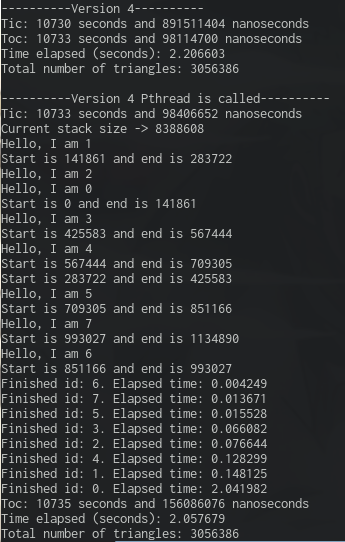
\includegraphics[height=.3\textheight, width=\textwidth, keepaspectratio]{assets/load_pthreads.png}
    \caption{Load balancing pthreads, static scheduling. Matrix com-Youtube.mtx}
\end{figure}


\end{document}
